% Provenance (never printed): old premiere S material on the formation of fossil
% fuels (preserved organic matter, burial, oil window, migration, trap, coal).
% Burial history of the invented Merrow Basin from figdata/grade-11/oil_window.py
% (constant geotherm, no compaction). Rifts and passive margins after the USGS
% West-Central Coastal Province fact sheet (2023-3028). Folds are defined in
% g12.02 mountain-building (Sync 0): the anticline is told in prose here, never
% defined. Sedimentary basins compared, diagenesis: Year 1/2.
\chapter{De geologie van steenkool, olie en gas}\label{ch:g11:fossil-fuel-geology}

Een plaat zwarte schalie uit een oude kolenmijn in Pennsylvania draagt de
bladeren van varenachtige planten, platgedrukt en zilverig tegen het donkere gesteente. Ze
groeiden meer dan driehonderd miljoen jaar geleden in een moeras, in het
Carboon; begraven voordat ze konden rotten, behielden ze hun vorm, en de
koolstof van de moerasplanten werd \omterm{def:g11:fossil-fuel-geology:coal}{steenkool}. Olie en gas, die vandaag worden opgepompt vanaf
platforms op zee, hebben dezelfde soort oorsprong: de resten van levende
wezens die aan afbraak ontsnapten en daarna werden begraven en verhit. Dit hoofdstuk
volgt die begraven koolstof van het moeras en de zeebodem tot de \omterm{def:g11:fossil-fuel-geology:coal}{steenkoollaag}
en het olieveld.
% ledger: photo:g11-fossil-plants, ics:base.Carboniferous, ics:base.Permian, earle:coal-formation, earle:organic-preservation

\begin{omfigure}
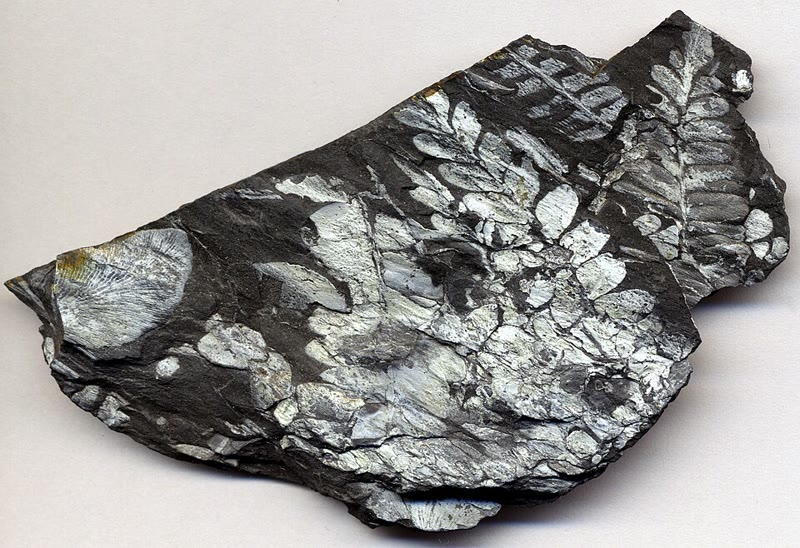
\includegraphics[height=4.4cm]{images/book2/g11-stjohn-fossil-plants.jpg}\hspace{0.03\linewidth}%
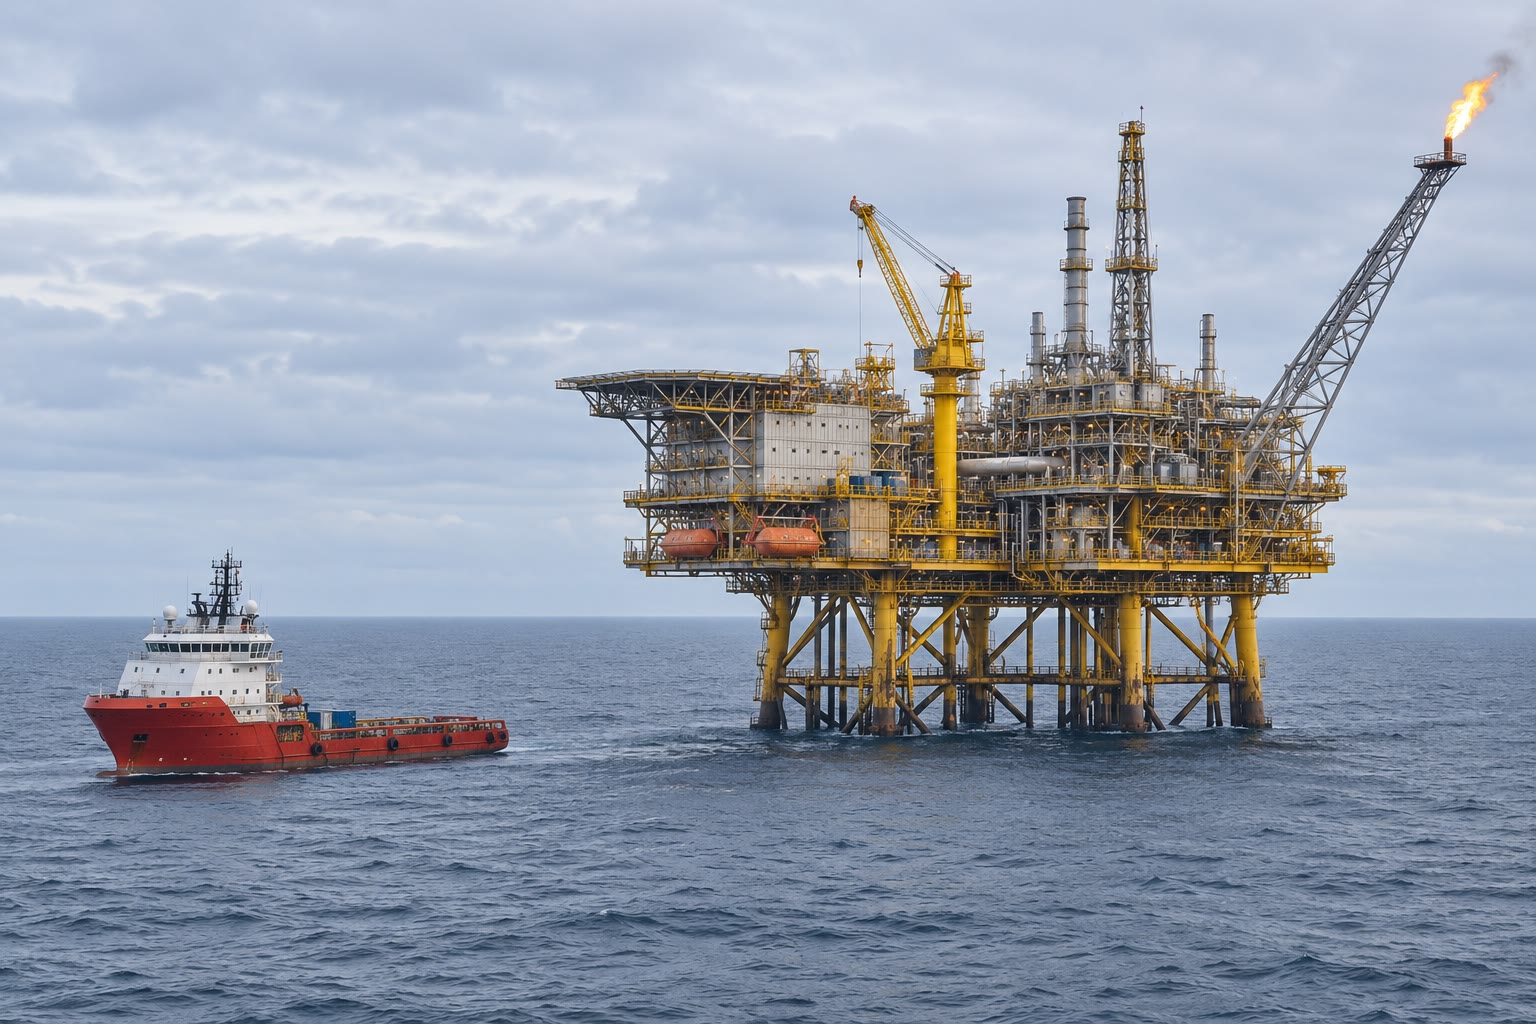
\includegraphics[height=4.4cm]{images/book2/ai/g11-offshore-platform.jpg}

{\small Links: fossiele plantenbladeren in koolstofrijke schalie uit een oude
kolenmijn, Pennsylvania, Carboon; de plaat is ongeveer \qty{10}{cm} breed.
Foto James St.~John (CC~BY~2.0). Rechts: een productieplatform voor olie en gas
op zee (AI-illustratie).}
\end{omfigure}
% ledger: photo:g11-fossil-plants

\begin{recall}
\omterm{def:g11:fossil-fuel-geology:coal}{Steenkool}, olie en aardgas zijn fossiele brandstoffen: olie en gas zijn mengsels van
koolwaterstoffen, verbindingen van koolstof en waterstof, en het verbranden van een fossiele brandstof
levert energie en koolstofdioxide op (de scheikundeboeken). Planten en algen
maken organisch materiaal uit koolstofdioxide en water door fotosynthese (de
biologieboeken). \omterm{def:g11:fossil-fuel-geology:coal}{Steenkool}, olie en gas komen van organisch materiaal dat in
sedimenten is begraven, en ze worden opgeslagen in sedimentaire gesteenten (Boek 1, jaar 9). Een gesteente
is poreus wanneer het lege ruimten bevat, doorlatend wanneer water erdoorheen kan
stromen (Boek 1, jaar 6). De temperatuur stijgt met de diepte langs de \omterm{def:g11:lithosphere-asthenosphere:geotherm}{geotherm},
met 25 tot \qty{30}{\degreeCelsius} per kilometer in de eerste kilometers
(\cref{ch:g11:lithosphere-asthenosphere}).
\end{recall}
% ledger: usgs:gradient-29, earle:organic-preservation

\section{Organisch materiaal bewaren}

Het meeste organische materiaal wordt nooit een brandstof. Een dood blad of een dode alg wordt
opgegeten door dieren en bacteriën of reageert met de zuurstof van de lucht: binnen
weken of jaren is zijn koolstof als koolstofdioxide naar de atmosfeer teruggekeerd.
Organisch materiaal overleeft alleen waar het van zuurstof is afgesloten --- op de
bodem van een stilstaand moeras, of op een zee- of meerbodem waarvan het water geen
zuurstof bevat. Daar begraven onder meer sediment kan het tientallen of
honderden miljoenen jaren bewaard blijven.
% ledger: earle:organic-preservation

\omterm{def:g11:fossil-fuel-geology:coal}{Steenkool} komt vooral van landplanten die zich in moerassen opstapelden. Olie en gas komen
vooral van de microscopisch kleine algen en ander plankton van de zee: waar het
oppervlaktewater heel productief is, regent dood plankton op de zeebodem
snel genoeg om voor een deel aan afbraak te ontsnappen, en wordt het in de modder begraven.
% ledger: earle:coal-formation, earle:oil-window

\begin{definition}[Brongesteente; kerogeen]\label{def:g11:fossil-fuel-geology:source-rock}
\emph{Kerogeen}\index{kerogeen} is het organische materiaal dat verspreid zit in een
sedimentair gesteente, in kleine deeltjes die niet oplossen in organische
oplosmiddelen. Een \emph{brongesteente}\index{brongesteente} is een sedimentair gesteente dat rijk
is aan kerogeen, en waarin olie en gas ontstaan wanneer het wordt begraven en verhit.
\end{definition}
% ledger: peters08:kerogen, earle:migration-traps

De meeste \omterm{def:g11:fossil-fuel-geology:source-rock}{brongesteenten} zijn schalies en kleistenen, afgezet als modder die rijk is aan
organisch materiaal. Dicht bij het oppervlak blijft hun \omterm{def:g11:fossil-fuel-geology:source-rock}{kerogeen} vast: bacteriën die
zonder zuurstof leven, zetten een deel van het organische materiaal om in methaan, maar het meeste
van dat methaan ontsnapt terug naar het oppervlak. Olie maken vraagt warmte, en warmte vraagt diepte.
% ledger: earle:oil-window, peters08:kerogen

\section{Begraving en rijping}

\begin{definition}[Sedimentair bekken]\label{def:g11:fossil-fuel-geology:basin}
Een \emph{sedimentair bekken}\index{sedimentair bekken} is een gebied van de korst
dat over miljoenen jaren daalt, zodat er sedimenten in worden opgestapeld, vaak
verscheidene kilometers dik.
\end{definition}
% ledger: usgs23:rift-salt

In een dalend bekken wordt elke laag steeds dieper begraven onder de lagen
die zich erbovenop opstapelen. Terwijl ze naar beneden gaat, volgt ze de \omterm{def:g11:lithosphere-asthenosphere:geotherm}{geotherm}: ze wordt
verhit. Haar \omterm{def:g11:fossil-fuel-geology:source-rock}{kerogeen} wordt langzaam gekookt, zijn grote moleculen worden gebroken tot de
kleinere van olie en gas.
% ledger: earle:oil-window

\begin{definition}[Rijping; olievenster; gasvenster]\label{def:g11:fossil-fuel-geology:oil-window}
De \emph{rijping}\index{rijping} van een \omterm{def:g11:fossil-fuel-geology:source-rock}{brongesteente} is de
omzetting van zijn \omterm{def:g11:fossil-fuel-geology:source-rock}{kerogeen} in olie en gas terwijl het wordt begraven en verhit.
Het \emph{olievenster}\index{olievenster} is het temperatuurbereik, van
ongeveer 60 tot \qty{120}{\degreeCelsius}, waarin het \omterm{def:g11:fossil-fuel-geology:source-rock}{kerogeen} vooral olie vormt.
Boven ongeveer \qty{120}{\degreeCelsius}, in het
\emph{gasvenster}\index{gasvenster}, vormt het vooral methaan.
\end{definition}
% ledger: earle:oil-window, magoon00:tps

Omdat de temperatuur met de diepte stijgt, is het \omterm{def:g11:fossil-fuel-geology:oil-window}{olievenster} ook een bereik van
diepten. Waar de \omterm{def:g11:lithosphere-asthenosphere:geotherm}{geotherm} een rechte lijn is, is het makkelijk te vinden.

\begin{proposition}[Diepte van het olievenster]\label{prop:g11:fossil-fuel-geology:window-depth}
Laat de temperatuur $T_0$ zijn aan het oppervlak en met de diepte $z$ stijgen met een
constante \omterm{def:g11:lithosphere-asthenosphere:geotherm}{geothermische gradiënt} $G$: $T = T_0 + G z$. Dan ligt het \omterm{def:g11:fossil-fuel-geology:oil-window}{olievenster}
tussen de diepten
\[
  z_{\text{boven}} = \frac{60 - T_0}{G}
  \qquad\text{en}\qquad
  z_{\text{onder}} = \frac{120 - T_0}{G},
\]
met temperaturen in \unit{\degreeCelsius}. Zijn dikte is $60/G$: hoe
steiler de \omterm{def:g11:lithosphere-asthenosphere:geotherm}{geotherm}, hoe ondieper en hoe dunner het venster.
\end{proposition}
% ledger: earle:oil-window

\begin{proof}
De bovenkant van het venster is de diepte waar $T_0 + G z = 60$, dat wil zeggen
$z = (60 - T_0)/G$; de onderkant is waar $T_0 + G z = 120$. Het verschil is
$(120 - 60)/G = 60/G$.
\end{proof}

Met een oppervlak van \qty{20}{\degreeCelsius} en een gradiënt van
\qty{30}{\degreeCelsius} per kilometer ligt het \omterm{def:g11:fossil-fuel-geology:oil-window}{olievenster} tussen
$40/30 \approx \qty{1.3}{km}$ en $100/30 \approx \qty{3.3}{km}$. In boorgaten
in de Verenigde Staten is de gradiënt gemiddeld
\qty{29}{\degreeCelsius} per kilometer, \num{25} in het oosten en \num{34}
in het westen; een \omterm{def:g11:fossil-fuel-geology:source-rock}{brongesteente} moet meestal meer dan ongeveer
\qty{2}{km} diep begraven zijn voordat het olie maakt. Wanneer er geen meting van het \omterm{def:g11:fossil-fuel-geology:source-rock}{kerogeen}
beschikbaar is, hebben aardoliegeologen een \omterm{def:g11:fossil-fuel-geology:source-rock}{brongesteente} dat onder meer
dan ongeveer \qty{3}{km} jongere gesteenten ligt, als rijp beschouwd.
% values (oil_window.py): z_top_km 1.3333, z_base_km 3.3333
% ledger: usgs:gradient-29, earle:oil-window, magoon00:tps

\begin{omfigure}
\begin{tikzpicture}
\begin{axis}[omrecord, omage, omdepth, name=burial, width=0.54\linewidth, height=5.6cm,
  xmin=0, xmax=170, ymin=0, ymax=4.5, xlabel={ouderdom (miljoen jaar geleden)},
  ylabel={diepte (\unit{km})}, unbounded coords=jump, clip=false,
  xtick={0,20,...,160}, ytick={0,1,...,4}]
\fill[omProp!18] (axis cs:170,1.3333) rectangle (axis cs:0,3.3333);
\fill[omThm!12] (axis cs:170,3.3333) rectangle (axis cs:0,4.5);
\node[font=\scriptsize, anchor=west, text=omProp!80!black] at (axis cs:168,1.75) {olievenster};
\node[font=\scriptsize, anchor=west, text=omThm] at (axis cs:168,3.9) {gasvenster};
\node[font=\scriptsize, anchor=south west, text=black!60, inner sep=1pt] at (axis cs:168,1.3333) {\qty{60}{\degreeCelsius}};
\node[font=\scriptsize, anchor=south west, text=black!60, inner sep=1pt] at (axis cs:168,3.3333) {\qty{120}{\degreeCelsius}};
% computed in figdata/grade-11/oil_window.py (invented basin)
\addplot[black!45, line width=0.6pt] table[x=age, y=z150] {figdata/out/grade-11-oil_window-history.dat};
\addplot[black!45, line width=0.6pt] table[x=age, y=z120] {figdata/out/grade-11-oil_window-history.dat};
\addplot[black!45, line width=0.6pt] table[x=age, y=z95] {figdata/out/grade-11-oil_window-history.dat};
\addplot[black!45, line width=0.6pt] table[x=age, y=z66] {figdata/out/grade-11-oil_window-history.dat};
\addplot[black, line width=1.4pt] table[x=age, y=z165] {figdata/out/grade-11-oil_window-history.dat};
\draw[omDef, dashed, line width=0.8pt] (axis cs:80,0) -- (axis cs:80,4.5);
\node[font=\scriptsize, anchor=west, text=omDef, inner sep=1pt] at (axis cs:78,4.2) {anticlinaal ontstaat};
\fill[omThm] (axis cs:116.97,1.3333) circle (2pt);
\fill[omThm] (axis cs:51.24,3.3333) circle (2pt);
\node[font=\scriptsize, anchor=north east, inner sep=1pt] at (axis cs:100,2.3) {brongesteente};
\end{axis}
\begin{axis}[omrecord, omdepth, at={(burial.east)}, anchor=west, xshift=1.7cm, width=0.34\linewidth, height=5.6cm,
  xmin=15, xmax=50, ymin=0, ymax=7, xlabel={gradiënt (\unit{\degreeCelsius/km})},
  ylabel={diepte (\unit{km})}]
% computed in figdata/grade-11/oil_window.py (proposition, surface at 20 degC)
\addplot[name path=top, omProp, line width=1pt] table[x=G, y=z_top] {figdata/out/grade-11-oil_window-windows.dat};
\addplot[name path=base, omThm, line width=1pt] table[x=G, y=z_base] {figdata/out/grade-11-oil_window-windows.dat};
\addplot[omProp!18] fill between[of=top and base];
\node[font=\scriptsize] at (axis cs:40,1.75) {olievenster};
\node[font=\scriptsize, anchor=south, text=omProp!80!black] at (axis cs:42,0.95) {bovenkant};
\node[font=\scriptsize, anchor=north west, text=omThm] at (axis cs:24,4.6) {onderkant};
\end{axis}
\end{tikzpicture}

{\small Links: begravingsgeschiedenis van het Merrowbekken, een verzonnen bekken (berekend
model, compactie verwaarloosd). Elke lijn volgt één laag door de tijd, vanaf
de dag dat ze aan het oppervlak werd afgezet; de dikke lijn is het \omterm{def:g11:fossil-fuel-geology:source-rock}{brongesteente},
165 miljoen jaar geleden afgezet. Met een oppervlak van
\qty{20}{\degreeCelsius} en een gradiënt van \qty{30}{\degreeCelsius} per
kilometer is het \omterm{def:g11:fossil-fuel-geology:oil-window}{olievenster} de band tussen \num{1.3} en
\qty{3.3}{km}. De stippen markeren wanneer het \omterm{def:g11:fossil-fuel-geology:source-rock}{brongesteente} erin kwam en wanneer het
eruit ging, naar het \omterm{def:g11:fossil-fuel-geology:oil-window}{gasvenster}. Rechts: diepte van de bovenkant en de onderkant van het
\omterm{def:g11:fossil-fuel-geology:oil-window}{olievenster} tegen de \omterm{def:g11:lithosphere-asthenosphere:geotherm}{geothermische gradiënt} (oppervlak op
\qty{20}{\degreeCelsius}).}
\end{omfigure}
% values (oil_window.py): enter_oil_Ma 116.97, leave_oil_Ma 51.24, T_max 140 (20 Ma), T_today 125

Een diagram als dit heet een \emph{begravingsdiagram}: de ouderdom loopt van
links naar rechts naar vandaag, de diepte naar beneden. Het maakt van een kolom gesteenten,
laag voor laag gedateerd, een verhaal.

\begin{method}[Een begravingsdiagram lezen]\label{met:g11:fossil-fuel-geology:burial}
\begin{enumerate}
  \item Zoek de lijn van het \omterm{def:g11:fossil-fuel-geology:source-rock}{brongesteente}: ze begint aan het oppervlak op de
        dag dat het gesteente werd afgezet.
  \item Teken de bovenkant en de onderkant van het \omterm{def:g11:fossil-fuel-geology:oil-window}{olievenster}, als diepten, uit de
        \omterm{def:g11:lithosphere-asthenosphere:geotherm}{geotherm} (\cref{prop:g11:fossil-fuel-geology:window-depth}).
  \item Lees de ouderdom af waarop de lijn van het \omterm{def:g11:fossil-fuel-geology:source-rock}{brongesteente} de bovenkant van het
        venster snijdt: het \omterm{def:g11:fossil-fuel-geology:source-rock}{brongesteente} begint olie te maken. Lees de ouderdom af waarop ze
        de onderkant snijdt: vanaf dan maakt het gas.
  \item Vergelijk die ouderdommen met de ouderdom van de \omterm{def:g11:fossil-fuel-geology:trap}{val}: alleen olie en gas
        die zijn ontstaan nadat de \omterm{def:g11:fossil-fuel-geology:trap}{val} bestaat, kunnen erin worden vastgehouden.
\end{enumerate}
\end{method}
% ledger: magoon00:tps

In het Merrowbekken komt het \omterm{def:g11:fossil-fuel-geology:source-rock}{brongesteente} ongeveer 117 miljoen jaar geleden in het \omterm{def:g11:fossil-fuel-geology:oil-window}{olievenster}
en verlaat het dat ongeveer 51 miljoen jaar geleden; zijn diepste
begraving, \qty{4.0}{km} bij \qty{140}{\degreeCelsius}, komt 20 miljoen jaar
geleden, voordat opheffing en erosie het weer omhoogbrengen. Vandaag ligt het nog in het
\omterm{def:g11:fossil-fuel-geology:oil-window}{gasvenster}. Het weekendprobleem berekent deze ouderdommen.
% values (oil_window.py): enter_oil_Ma 116.97, leave_oil_Ma 51.24, z_max_km 4, T_max 140, T_today 125

\section{Van bron naar val}

Olie en gas zijn lichter dan water, en de poriën van begraven gesteenten zijn vol
water. Eenmaal gevormd worden ze uit het \omterm{def:g11:fossil-fuel-geology:source-rock}{brongesteente} geperst en kruipen ze omhoog,
door elk gesteente dat ze doorlaat.
% ledger: earle:migration-traps

\begin{definition}[Migratie]\label{def:g11:fossil-fuel-geology:migration}
\emph{Migratie}\index{migratie (van olie en gas)} is de langzame beweging van
olie en gas uit het \omterm{def:g11:fossil-fuel-geology:source-rock}{brongesteente} waarin ze zijn ontstaan, omhoog door
doorlatende gesteenten, aangedreven door hun lagere dichtheid dan het water eromheen.
\end{definition}
% ledger: earle:migration-traps

\begin{definition}[Reservoirgesteente; afdekgesteente]\label{def:g11:fossil-fuel-geology:reservoir}
Een \emph{reservoirgesteente}\index{reservoirgesteente} is een poreus en doorlatend
gesteente waarin olie en gas zich verzamelen: zijn poriën slaan ze op, en hun verbindingen
laten ze naar een put stromen. Een \emph{afdekgesteente}\index{afdekgesteente} is een
ondoorlatend gesteente boven het reservoir, waar olie en gas niet
doorheen kunnen.
\end{definition}
% ledger: earle:migration-traps, magoon00:tps

Zandstenen en sommige kalkstenen zijn goede reservoirs; kleistenen, schalies en
zout zijn goede \omterm{def:g11:fossil-fuel-geology:reservoir}{afdekgesteenten}. Waar niets ze tegenhoudt, bereiken olie en gas het
oppervlak, waar ze naar buiten sijpelen en worden geoxideerd: hun koolstof gaat terug naar de
atmosfeer. Ze verzamelen zich alleen waar een \omterm{def:g11:fossil-fuel-geology:reservoir}{afdekgesteente} zo is gevormd dat ze er
niet langs kunnen glippen.
% ledger: earle:migration-traps, magoon00:tps

\begin{definition}[Val]\label{def:g11:fossil-fuel-geology:trap}
Een \emph{val}\index{val (voor olie en gas)} is een opbouw van \omterm{def:g11:fossil-fuel-geology:reservoir}{reservoirgesteente}
en \omterm{def:g11:fossil-fuel-geology:reservoir}{afdekgesteente} die olie en gas op hun plaats houdt, doordat hij de weg omhoog aan elke kant afsluit.
\end{definition}
% ledger: earle:migration-traps

\begin{omfigure}
\begin{tikzpicture}[font=\footnotesize, scale=0.95,
    declare function={hz(\x,\c)=\c+0.1*\x+0.7*exp(-((\x-10)^2)/2.5);}]
  \colorlet{omOil}{green!45!black}\colorlet{omGas}{red!65}
  \fill[omLithShale!70!white] (0,0) rectangle (14,-6.3);
  % overburden: limestone above a sandstone
  \fill[omLithCongl!70!white] (0,0) -- (14,0) -- plot[domain=14:0, samples=80] (\x,{-2.4+0.06*\x+0.3*exp(-((\x-10)^2)/2.5)}) -- cycle;
  \fill[omLithSand!60!white] plot[domain=0:14, samples=80] (\x,{-2.4+0.06*\x+0.3*exp(-((\x-10)^2)/2.5)}) -- plot[domain=14:0, samples=80] (\x,{hz(\x,-3.7)}) -- cycle;
  % seal (mudstone)
  \fill[omLithShale] plot[domain=0:14, samples=80] (\x,{hz(\x,-3.7)}) -- plot[domain=14:0, samples=80] (\x,{hz(\x,-4.4)}) -- cycle;
  % reservoir sandstone
  \fill[omLithSand] plot[domain=0:14, samples=80] (\x,{hz(\x,-4.4)}) -- plot[domain=14:0, samples=80] (\x,{hz(\x,-5.0)}) -- cycle;
  % oil and gas in the crest of the anticline, above the spill depth
  \begin{scope}
    \clip plot[domain=0:14, samples=80] (\x,{hz(\x,-4.4)}) -- plot[domain=14:0, samples=80] (\x,{hz(\x,-5.0)}) -- cycle;
    \fill[omOil] (8,-2.97) rectangle (13,-2.6);
    \fill[omGas] (8,-2.81) rectangle (13,-2.6);
  \end{scope}
  % source rock (black shale)
  \fill[black!70] plot[domain=0:14, samples=80] (\x,{hz(\x,-5.0)}) -- plot[domain=14:0, samples=80] (\x,{hz(\x,-5.6)}) -- cycle;
  \foreach \c in {-3.7,-4.4,-5.0,-5.6}
    \draw[black!55, line width=0.4pt] plot[domain=0:14, samples=80] (\x,{hz(\x,\c)});
  \draw[black!55, line width=0.4pt] plot[domain=0:14, samples=80] (\x,{-2.4+0.06*\x+0.3*exp(-((\x-10)^2)/2.5)});
  \draw[black!70] (0,0) -- (14,0);
  % 60 degC isotherm
  \draw[omThm, dashed, line width=0.8pt] (0,-4.3) -- (14,-4.3);
  \node[anchor=north east, text=omThm, fill=omLithShale!70!white, inner sep=1pt] at (13.95,-4.35) {\qty{60}{\degreeCelsius}};
  % migration
  \foreach \s in {0,1}
    \draw[->, omDef, line width=1.1pt] (2.7+1.2*\s,{-5.1+0.12*\s}) -- (3.2+1.2*\s,{-4.55+0.12*\s});
  \draw[->, omDef, line width=1.1pt] (4.6,-4.3) .. controls (6.5,-4.1) and (8.3,-3.7) .. (9.45,-3.0);
  % labels
  \node[anchor=west, text=white] at (0.15,-5.25) {brongesteente};
  \node[anchor=west] at (5.2,-5.75) {rijp waar warmer dan \qty{60}{\degreeCelsius}};
  \node[anchor=west] at (0.15,-4.75) {reservoirgesteente};
  \node[anchor=west] at (0.15,-3.97) {afdekgesteente};
  \node[anchor=west] at (0.15,-0.4) {dekpakket};
  \node[anchor=north, text=omDef, fill=omLithShale, inner sep=1pt] at (6.2,-3.62) {migratie};
  \draw[black!60] (10.0,-2.72) -- (11.4,-1.95);
  \node[anchor=south west, fill=omLithSand!60!white, inner sep=1pt] at (11.4,-1.95) {gas};
  \draw[black!60] (10.6,-2.88) -- (12.3,-2.55);
  \node[anchor=west, fill=omLithShale, inner sep=1pt] at (12.3,-2.55) {olie};
  \draw[black!60] (12.0,-3.45) -- (12.8,-3.15);
  \node[anchor=south, fill=omLithShale, inner sep=1pt] at (12.85,-3.15) {water};
  \node[anchor=north] at (10,-1.0) {val: de boog van een anticlinaal};
\end{tikzpicture}

{\small Een \omterm{def:g11:fossil-fuel-geology:petroleum-system}{petroleumsysteem} (een tekening, niet op schaal). Het \omterm{def:g11:fossil-fuel-geology:source-rock}{brongesteente}, diep
links, ligt onder de isotherm van \qty{60}{\degreeCelsius} en maakt
olie; olie en gas bewegen eruit naar de zandsteen erboven en kruipen erlangs
omhoog, onder het \omterm{def:g11:fossil-fuel-geology:reservoir}{afdekgesteente} van kleisteen, naar de boog van een anticlinaal. Daar verzamelen ze zich
naar dichtheid: gas bovenaan, olie eronder, water onderaan. Het \omterm{def:g11:fossil-fuel-geology:petroleum-system}{dekpakket}
erbovenop begraaft het \omterm{def:g11:fossil-fuel-geology:source-rock}{brongesteente} diep genoeg om het te laten rijpen.}
\end{omfigure}
% ledger: earle:migration-traps, magoon00:tps, earle:oil-window

In een \omterm{def:g11:fossil-fuel-geology:trap}{val} sorteren de vloeistoffen zich naar dichtheid: gas bovenaan, olie eronder,
water onderaan. De eenvoudigste \omterm{def:g11:fossil-fuel-geology:trap}{val} is een anticlinaal, een boog in
de lagen (plooien zijn het onderwerp van \cref{ch:g12:mountain-building}). Breuken,
zoutkoepels en veranderingen in de gesteenten zelf maken ook vallen.
% ledger: earle:migration-traps

\begin{omfigure}
\begin{tikzpicture}[font=\footnotesize, scale=0.78]
  \colorlet{omOil}{green!45!black}\colorlet{omGas}{red!65}
  % (a) anticline
  \begin{scope}
    \fill[omLithShale] (0,0) rectangle (4,3);
    \fill[omLithSand] plot[domain=0:4, samples=50] (\x,{1.0+1.0*exp(-((\x-2)^2)/1.2)}) -- plot[domain=4:0, samples=50] (\x,{1.5+1.0*exp(-((\x-2)^2)/1.2)}) -- cycle;
    \begin{scope}
      \clip plot[domain=0:4, samples=50] (\x,{1.0+1.0*exp(-((\x-2)^2)/1.2)}) -- plot[domain=4:0, samples=50] (\x,{1.5+1.0*exp(-((\x-2)^2)/1.2)}) -- cycle;
      \fill[omOil] (0,1.75) rectangle (4,3); \fill[omGas] (0,2.25) rectangle (4,3);
    \end{scope}
    \draw[black!50] (0,0) rectangle (4,3);
    \node[anchor=north, text height=1.6ex, text depth=0.3ex] at (2,-0.05) {(a) anticlinaal};
  \end{scope}
  % (b) fault
  \begin{scope}[xshift=4.6cm]
    \fill[omLithShale] (0,0) rectangle (4,3);
    \begin{scope}
      \clip (0,0) -- (2.9,0) -- (2.3,3) -- (0,3) -- cycle;
      \fill[omLithSand] (0,0.6) -- (4,1.8) -- (4,2.3) -- (0,1.1) -- cycle;
      \clip (0,0.6) -- (4,1.8) -- (4,2.3) -- (0,1.1) -- cycle;
      \fill[omOil] (0,1.45) rectangle (4,3); \fill[omGas] (0,1.75) rectangle (4,3);
    \end{scope}
    \begin{scope}
      \clip (2.9,0) -- (4,0) -- (4,3) -- (2.3,3) -- cycle;
      \fill[omLithSand] (0,-0.6) -- (4,0.6) -- (4,1.1) -- (0,-0.1) -- cycle;
    \end{scope}
    \draw[black, line width=1pt] (2.9,0) -- (2.3,3);
    \draw[black!50] (0,0) rectangle (4,3);
    \node[anchor=north, text height=1.6ex, text depth=0.3ex] at (2,-0.05) {(b) breuk};
  \end{scope}
  % (c) salt dome
  \begin{scope}[xshift=9.2cm]
    \fill[omLithShale] (0,0) rectangle (4,3);
    \fill[omLithSand] (0,0.9) -- (1.0,1.2) -- (1.4,1.9) -- (1.4,2.4) -- (1.0,1.7) -- (0,1.4) -- cycle;
    \fill[omLithSand] (4,0.9) -- (3.0,1.2) -- (2.6,1.9) -- (2.6,2.4) -- (3.0,1.7) -- (4,1.4) -- cycle;
    \begin{scope}
      \clip (0,0.9) -- (1.0,1.2) -- (1.4,1.9) -- (1.4,2.4) -- (1.0,1.7) -- (0,1.4) -- cycle;
      \fill[omOil] (0,1.65) rectangle (1.4,3); \fill[omGas] (0,2.05) rectangle (1.4,3);
    \end{scope}
    \begin{scope}
      \clip (4,0.9) -- (3.0,1.2) -- (2.6,1.9) -- (2.6,2.4) -- (3.0,1.7) -- (4,1.4) -- cycle;
      \fill[omOil] (2.6,1.65) rectangle (4,3); \fill[omGas] (2.6,2.05) rectangle (4,3);
    \end{scope}
    \fill[omLithEvap, draw=black!60] (1.4,0) -- (1.4,2.4) .. controls (1.4,2.85) and (2.6,2.85) .. (2.6,2.4) -- (2.6,0) -- cycle;
    \node at (2,1.0) {zout};
    \draw[black!50] (0,0) rectangle (4,3);
    \node[anchor=north, text height=1.6ex, text depth=0.3ex] at (2,-0.05) {(c) zoutkoepel};
  \end{scope}
  % (d) stratigraphic
  \begin{scope}[xshift=13.8cm]
    \fill[omLithShale] (0,0) rectangle (4,3);
    \fill[omLithSand] (0,0.6) -- (3.5,1.95) -- (0,1.3) -- cycle;
    \begin{scope}
      \clip (0,0.6) -- (3.5,1.95) -- (0,1.3) -- cycle;
      \fill[omOil] (0,1.45) rectangle (4,3); \fill[omGas] (0,1.7) rectangle (4,3);
    \end{scope}
    \draw[black!50] (0,0) rectangle (4,3);
    \node[anchor=north, text height=1.6ex, text depth=0.3ex] at (2,-0.05) {(d) uitwigging};
  \end{scope}
\end{tikzpicture}

{\small Vier soorten vallen (tekeningen, niet op schaal): reservoirzandsteen in
geel, afdekkende kleisteen in grijsgroen, olie in groen, gas in rood. (a) De
boog van een anticlinaal. (b) Een scheefgesteld reservoir dat door een breuk wordt afgesneden, tegen een
kleisteen aan de andere kant. (c) Lagen die omhoog zijn gebogen tegen een opstijgende zoutkoepel.
(d) Een zandsteen die hellingopwaarts in kleisteen uitwigt, een \omterm{def:g11:fossil-fuel-geology:trap}{val} die ontstaat door een
verandering in de gesteenten zelf.}
\end{omfigure}
% ledger: earle:migration-traps

\begin{example}[Een val in een anticlinaal]\label{ex:g11:fossil-fuel-geology:anticline}
Een seismisch onderzoek brengt de bovenkant van een zandsteen onder een afdeklaag van kleisteen in kaart. Die vormt een
boog waarvan de top \qty{1800}{m} onder het oppervlak ligt. Rond de top ligt de
diepste hoogtelijn die nog helemaal rondom sluit, op
\qty{2050}{m}; daaronder is de zandsteen opzij open. Een put op de top
vindt gas tot \qty{1880}{m}. Hoe hoog kan de kolom olie en gas zijn die de
\omterm{def:g11:fossil-fuel-geology:trap}{val} kan bevatten, en hoe dik is de olie?

\emph{Oplossing.} Olie en gas vullen de boog van de top naar beneden; wat
onder de laatste gesloten hoogtelijn zakt, loopt opzij weg, bij het
\emph{overlooppunt}, en migreert verder. De kolom is hoogstens
$2050 - 1800 = \qty{250}{m}$ hoog. Als de \omterm{def:g11:fossil-fuel-geology:trap}{val} vol is, vult gas de bovenste
$1880 - 1800 = \qty{80}{m}$ en olie de volgende $2050 - 1880 = \qty{170}{m}$,
met water eronder.
\end{example}
% invented numbers; ledger: earle:migration-traps

Elk van de onderdelen --- een \omterm{def:g11:fossil-fuel-geology:source-rock}{brongesteente}, een reservoir, een \omterm{def:g11:fossil-fuel-geology:reservoir}{afdekgesteente}, de gesteenten erbovenop
die het \omterm{def:g11:fossil-fuel-geology:source-rock}{brongesteente} begraven, een \omterm{def:g11:fossil-fuel-geology:trap}{val} --- is nodig, en ze moeten in de
juiste volgorde komen.

\begin{definition}[Petroleumsysteem]\label{def:g11:fossil-fuel-geology:petroleum-system}
Een \emph{petroleumsysteem}\index{petroleumsysteem} is een lichaam rijp \omterm{def:g11:fossil-fuel-geology:source-rock}{brongesteente}
samen met alle olie en gas die eruit zijn voortgekomen, en de elementen
en processen die ze nodig hebben: het \omterm{def:g11:fossil-fuel-geology:source-rock}{brongesteente}, het \omterm{def:g11:fossil-fuel-geology:reservoir}{reservoirgesteente}, het \omterm{def:g11:fossil-fuel-geology:reservoir}{afdekgesteente} en
het \emph{dekpakket}\index{dekpakket} (de gesteenten erboven, die het
\omterm{def:g11:fossil-fuel-geology:source-rock}{brongesteente} begraven), en de vorming van vallen, het ontstaan, de \omterm{def:g11:fossil-fuel-geology:migration}{migratie} en de
ophoping van olie en gas.
\end{definition}
% ledger: magoon00:tps

De volgorde telt het meest. Een \omterm{def:g11:fossil-fuel-geology:trap}{val} die ontstaat nadat de olie voorbij is, vangt
niets: het begravingsdiagram dateert het ontstaan van olie, de geschiedenis
van de plooien en breuken dateert de \omterm{def:g11:fossil-fuel-geology:trap}{val}, en het \omterm{def:g11:fossil-fuel-geology:petroleum-system}{petroleumsysteem} werkt alleen
als de \omterm{def:g11:fossil-fuel-geology:trap}{val} er eerst was. Aardoliegeologen noemen het tijdstip dat ontstaan, \omterm{def:g11:fossil-fuel-geology:migration}{migratie} en
ophoping het best samen laat zien ook het \emph{kritieke
moment}.
% ledger: magoon00:tps

\section{Waar olie en gas zich verzamelen}

Waar komt een \omterm{def:g11:fossil-fuel-geology:petroleum-system}{petroleumsysteem} samen? Het heeft een bekken nodig dat lang
daalt, zuurstofarm water om organisch materiaal te bewaren, en \omterm{def:g11:fossil-fuel-geology:reservoir}{afdekgesteenten}. Rifts
en de continentranden waartoe ze uitgroeien, hebben alle drie.
% ledger: usgs23:rift-salt

Wanneer een continent begint te splijten, zoals Afrika vandaag langs de Oost-Afrikaanse
Rift (Boek 1, jaar 7), rekt zijn korst uit en breekt ze in blokken
langs \omterm{def:g11:ocean-ridges:normal-fault}{afschuivingen} (\cref{ch:g11:ocean-ridges}). Sommige blokken zakken, andere
kantelen, en de troggen ertussen vullen zich met sedimenten, vaak verscheidene
kilometers dik, en met meren, waarvan de modder die rijk is aan organisch materiaal
\omterm{def:g11:fossil-fuel-geology:source-rock}{brongesteente} kan worden. Wanneer
de uitrekking stopt, koelt de verdunde korst af en blijft ze langzaam dalen, zodat
het bekken zich blijft vullen. Als de zee dan een bekken binnenstroomt dat maar
gedeeltelijk met de oceaan is verbonden, en verdampt, laat ze dikke lagen
zout achter. Zodra de rift tot een oceaan is opengegaan, worden zijn randen passieve
randen: continentranden binnen een plaat, ver van elke plaatgrens, die
blijven dalen en sediment van het land ontvangen.
% ledger: usgs23:rift-salt, usgs:pangaea-breakup

\begin{omfigure}
\begin{tikzpicture}[font=\footnotesize, x=1cm, y=0.8cm]
  \fill[omLithShale] (0,0.25) -- (1.5,0) -- (7,-0.4) -- (10,-2.2) -- (14,-2.6) -- (14,-8.0) -- (0,-8.0) -- cycle;
  % sea and land
  \fill[omSea] (1.5,0) -- (14,0) -- (14,-2.6) -- (10,-2.2) -- (7,-0.4) -- cycle;
  \draw[omRiver!60, line width=0.6pt] (1.5,0) -- (14,0);
  % marine sediments above the salt
  \fill[omLithShale] (0,0.25) -- (1.5,0) -- (7,-0.4) -- (10,-2.2) -- (14,-2.6) -- (14,-4.95) -- (11.2,-4.5) -- (11.2,-3.74) -- (0,-2.4) -- cycle;
  \fill[omLithSand] (0,-0.9) -- (6,-1.45) -- (10,-2.75) -- (14,-3.3) -- (14,-3.6) -- (10,-3.05) -- (6,-1.75) -- (0,-1.2) -- cycle;
  % salt layer and a salt dome
  \fill[omLithEvap, draw=black!50] (1.2,-2.25) -- (11.2,-3.74) -- (11.2,-4.14) -- (1.2,-2.65) -- cycle;
  \fill[omLithEvap, draw=black!50] (7.0,-3.0) .. controls (7.3,-2.6) and (7.25,-1.9) .. (7.2,-1.6)
     .. controls (7.4,-1.2) and (8.2,-1.2) .. (8.4,-1.6)
     .. controls (8.35,-2.1) and (8.3,-2.7) .. (8.7,-3.25) -- cycle;
  % continental crust with tilted blocks
  \fill[omLithGranite] (0,-2.75) -- (2.5,-3.0) -- (4.85,-4.6) -- (5.0,-3.4) -- (7.35,-5.0) -- (7.5,-3.75) -- (9.85,-5.3) -- (10.0,-4.1) -- (11.2,-5.0) -- (11.2,-6.0) -- (0,-7.6) -- cycle;
  % rift fill: lake shales (source rocks) in the half-grabens
  \fill[black!65] (2.5,-3.0) -- (4.85,-4.6) -- (5.0,-3.4) -- (4.0,-3.25) -- cycle;
  \fill[black!65] (5.0,-3.4) -- (7.35,-5.0) -- (7.5,-3.75) -- (6.5,-3.6) -- cycle;
  \fill[black!65] (7.5,-3.75) -- (9.85,-5.3) -- (10.0,-4.1) -- (9.0,-3.95) -- cycle;
  \fill[black!65] (2.5,-3.0) -- (4.0,-3.25) -- (5.0,-3.4) -- (6.5,-3.6) -- (7.5,-3.75) -- (9.0,-3.95) -- (10.0,-4.1) -- (11.2,-4.3) -- (11.2,-4.14) -- (1.2,-2.65) -- (1.2,-2.87) -- cycle;
  \draw[black!70, line width=0.8pt] (4.85,-4.6) -- (5.0,-3.4) (7.35,-5.0) -- (7.5,-3.75) (9.85,-5.3) -- (10.0,-4.1);
  % oceanic crust and mantle
  \fill[omLithBasalt] (11.2,-4.5) -- (14,-4.95) -- (14,-6.0) -- (11.2,-6.0) -- cycle;
  \fill[omLithPeridotite] (0,-7.6) -- (11.2,-6.0) -- (14,-6.0) -- (14,-8.0) -- (0,-8.0) -- cycle;
  % oil beside the salt dome
  \fill[green!45!black] (6.85,-1.5) -- (7.22,-1.65) -- (7.22,-1.95) -- (6.85,-1.75) -- cycle;
  \draw[black!60] (0,-8.0) rectangle (14,1.0);
  % labels
  \node[anchor=west] at (11.5,-1.2) {zee};
  \node[anchor=south west] at (0.1,0.3) {land};
  \node[anchor=west, fill=omLithShale, inner sep=1pt] at (2.2,-0.45) {mariene sedimenten};
  \node[anchor=west, fill=omLithEvap, inner sep=1pt] at (9.0,-1.25) {zoutkoepel};
  \draw[black!60] (8.4,-1.4) -- (9.0,-1.25);
  \node[anchor=east, fill=omLithShale, inner sep=1pt] at (6.6,-2.1) {olie};
  \draw[black!60] (6.6,-2.1) -- (6.95,-1.75);
  \node[anchor=west, fill=omLithShale, inner sep=1pt] at (11.4,-3.35) {zout (afdekking)};
  \draw[black!60] (10.8,-3.7) -- (11.4,-3.35);
  \node[anchor=west, align=left] at (0.3,-4.7) {meerschalies\\(brongesteenten)};
  \draw[black!60] (2.75,-4.45) -- (4.4,-3.8);
  \node[anchor=north, align=center] at (4.0,-5.6) {uitgerekte continentale korst:\\gekantelde blokken en afschuivingen};
  \node[anchor=north, align=center] at (12.6,-5.05) {oceanische korst};
  \node[anchor=north] at (6,-7.35) {mantel};
\end{tikzpicture}

{\small Een passieve rand die op een oude rift is gebouwd (een tekening, niet op schaal, diepten
overdreven). In de rift bevatten gekantelde blokken continentale korst, begrensd door
\omterm{def:g11:ocean-ridges:normal-fault}{afschuivingen}, meerschalies, de \omterm{def:g11:fossil-fuel-geology:source-rock}{brongesteenten}. Een zoutlaag, afgezet
toen de jonge zee verdampte, dekt ze af; daarboven stapelen mariene sedimenten zich
op terwijl de rand daalt. Zout, lichter dan de sedimenten eromheen, stijgt op
in koepels die de lagen tot vallen buigen.}
\end{omfigure}
% ledger: usgs23:rift-salt, earle:migration-traps

De randen van de Zuid-Atlantische Oceaan zijn zo opgebouwd. Afrika en Zuid-Amerika
begonnen in het Laat-Trias of Vroeg-Jura uit elkaar te gaan. Voor de kust van
het westen van Centraal-Afrika vulden de rifttroggen zich met verscheidene kilometers
sediment, waaronder meerschalies tot \qty{600}{m} dik met tot
\qty{20}{\percent} organische koolstof naar massa. In het Vroeg-Krijt begon de zee
keer op keer binnen te stromen, en verdampte ze, waarbij ze meer dan een
kilometer zout achterliet; waar het zout op zijn plaats is gebleven, dekt het de olie en het
gas van de gesteenten eronder af. In de Golf van Mexico is zout dat lichter is dan de
sedimenten eromheen in koepels opgestegen, en de lagen die ertegen zijn gebogen,
zijn vallen.
% ledger: usgs23:rift-salt, earle:migration-traps

\section{Steenkool}

\omterm{def:g11:fossil-fuel-geology:coal}{Steenkool} ontstaat op het land, vooral in moerassen langs rivieren en delta's, in vochtige
klimaten van tropisch tot gematigd, waar planten snel groeien en hun resten
in stilstaand, zuurstofarm water vallen. In eeuwen tot millennia stapelen ze zich
op als veen. Wanneer een rivier van loop verandert, of de zee stijgt, begraven zand en modder
het veen; dieper begraven wordt het samengeperst en verhit.
% ledger: earle:coal-formation

\begin{definition}[Steenkool; inkoling; inkolingsgraad]\label{def:g11:fossil-fuel-geology:coal}
\emph{Steenkool}\index{steenkool} is een sedimentair gesteente dat vooral bestaat uit de resten van
landplanten, rijk aan koolstof. \emph{Inkoling}\index{inkoling} is de
omzetting van veen in steenkool en van steenkool in rijkere steenkool, door begraving en
verhitting. De \emph{inkolingsgraad}\index{inkolingsgraad} van een steenkool is hoe ver
de inkoling is gevorderd: van bruinkool via subbitumineuze en bitumineuze
kool tot antraciet stijgt het koolstofgehalte.
\end{definition}
% ledger: earle:coal-formation, eia:coal-carbon

Bruinkool ontstaat op diepten van een paar honderd meter tot ongeveer \qty{1.5}{km},
tot ongeveer \qty{50}{\degreeCelsius}; \omterm{def:g11:fossil-fuel-geology:coal}{bitumineuze kool} tussen 1 en
\qty{5}{km}, tot ongeveer \qty{150}{\degreeCelsius}; antraciet voorbij
\qty{5}{km} en \qty{150}{\degreeCelsius}. Naarmate de \omterm{def:g11:fossil-fuel-geology:coal}{inkolingsgraad} stijgt, maakt koolstof
een steeds groter deel van de kool uit: ongeveer
25 tot \qty{35}{\percent} in bruinkool, tot 86 à \qty{97}{\percent} in
antraciet. Methaan dat onderweg ontstaat, blijft in de poriën van de kool, en
daarom kan een kolenmijn explosief gas bevatten. Het vormen van een \omterm{def:g11:fossil-fuel-geology:coal}{steenkoollaag} duurt miljoenen
jaren.
% ledger: earle:coal-formation, eia:coal-carbon

\begin{omfigure}
\begin{tikzpicture}
\begin{axis}[omrecord, xbar, name=rank, width=0.5\linewidth, height=4.6cm, xmin=0, xmax=100,
  ymin=0.4, ymax=4.6, ytick={1,2,3,4},
  yticklabels={bruinkool, subbitumineus, bitumineus, antraciet},
  xlabel={koolstofgehalte (\unit{\percent})}, ymajorgrids=false]
% ledger: eia:coal-carbon
\fill[omProp!60!black!35] (axis cs:25,0.7) rectangle (axis cs:35,1.3);
\fill[omProp!70!black!55] (axis cs:35,1.7) rectangle (axis cs:45,2.3);
\fill[black!60] (axis cs:45,2.7) rectangle (axis cs:86,3.3);
\fill[black!85] (axis cs:86,3.7) rectangle (axis cs:97,4.3);
\node[font=\scriptsize, anchor=west] at (axis cs:36,1) {25--35};
\node[font=\scriptsize, anchor=west] at (axis cs:46,2) {35--45};
\node[font=\scriptsize, anchor=east, text=white] at (axis cs:85,3) {45--86};
\node[font=\scriptsize, anchor=east] at (axis cs:85,4) {86--97};
\end{axis}
\node[anchor=west] at ([xshift=0.6cm]rank.east) {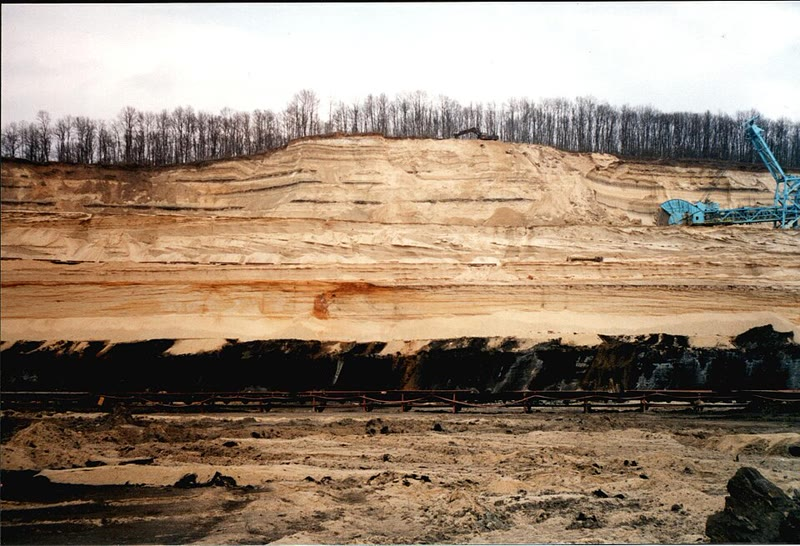
\includegraphics[height=4.0cm]{images/book2/g11-usgs-lignite-bed.jpg}};
\end{tikzpicture}

\medskip
\makebox[0.32\linewidth]{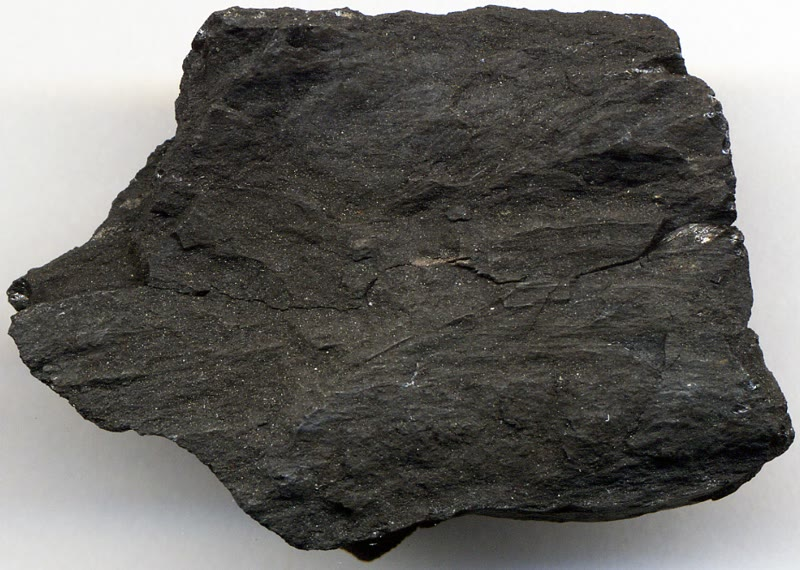
\includegraphics[height=3.2cm]{images/book2/g11-stjohn-lignite.jpg}}\hfill
\makebox[0.32\linewidth]{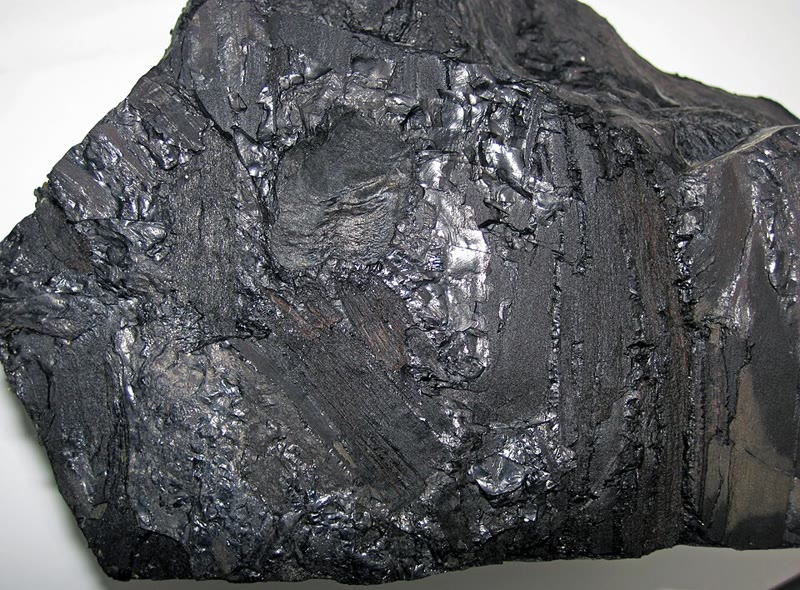
\includegraphics[height=3.2cm]{images/book2/g11-stjohn-bituminous.jpg}}\hfill
\makebox[0.32\linewidth]{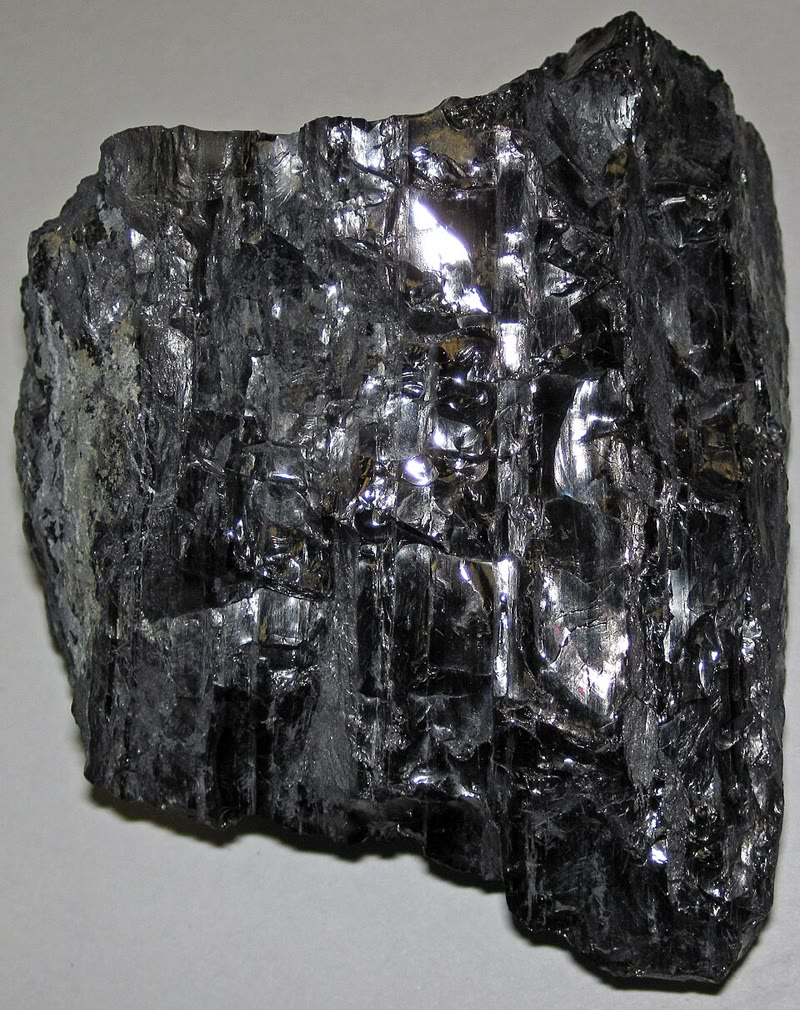
\includegraphics[height=3.2cm]{images/book2/g11-stjohn-anthracite.jpg}}

{\small Linksboven: koolstofgehalte van de rangen van \omterm{def:g11:fossil-fuel-geology:coal}{steenkool}. Gegevens: U.S. Energy
Information Administration. Rechtsboven: een bruinkoollaag, de zwarte band
onder lichte zanden, blootgelegd in een mijn in Roemenië; foto U.S. Geological
Survey (publiek domein). Onder, van links: bruinkool, ongeveer \qty{4.5}{cm}
breed, bruinzwart en dof; \omterm{def:g11:fossil-fuel-geology:coal}{bitumineuze kool}, met platgedrukte
plantenfragmenten; antraciet, zwart en glazig. Foto's James St.~John
(CC~BY~2.0).}
\end{omfigure}
% ledger: eia:coal-carbon, photo:g11-lignite-bed, photo:g11-coal-ranks

Veen verliest onderweg het grootste deel van zijn volume. In een \omterm{def:g11:fossil-fuel-geology:coal}{steenkoollaag} in het midden van Utah
geeft de vergelijking van het veen dat door een oude rivierbedding is weggesneden met de kool die
ernaast ontbreekt, een verhouding van diktes van ongeveer $11{:}1$: elke meter van die
\omterm{def:g11:fossil-fuel-geology:coal}{bitumineuze kool} was ooit zo'n elf meter veen.
% ledger: ryer80:peat-coal

\section{Oefeningen}

\begin{exercise}[$\star$]\label{exo:g11:fossil-fuel-geology:1}
Zet de stappen op volgorde die van plankton tot olie in een \omterm{def:g11:fossil-fuel-geology:trap}{val} leiden: \omterm{def:g11:fossil-fuel-geology:migration}{migratie};
\omterm{def:g11:fossil-fuel-geology:oil-window}{rijping} in het \omterm{def:g11:fossil-fuel-geology:oil-window}{olievenster}; begraving onder jongere sedimenten; dood plankton
bezinkt op een zuurstofarme zeebodem; olie verzamelt zich onder een \omterm{def:g11:fossil-fuel-geology:reservoir}{afdekgesteente}; het organische
materiaal wordt \omterm{def:g11:fossil-fuel-geology:source-rock}{kerogeen} in een modder.
\end{exercise}

\begin{exercise}[$\star$]\label{exo:g11:fossil-fuel-geology:2}
Zeg voor elk gesteente of het eerder een \omterm{def:g11:fossil-fuel-geology:source-rock}{brongesteente}, een \omterm{def:g11:fossil-fuel-geology:reservoir}{reservoirgesteente}
of een \omterm{def:g11:fossil-fuel-geology:reservoir}{afdekgesteente} is: (1) een donkere schalie die rijk is aan organisch materiaal; (2) een goed gesorteerde
zandsteen met verbonden poriën; (3) een zoutlaag; (4) een kleisteen zonder
organisch materiaal; (5) een kalksteen vol open holten.
\end{exercise}

\begin{exercise}[$\star$]\label{exo:g11:fossil-fuel-geology:3}
In een bekken is het oppervlak \qty{10}{\degreeCelsius} en de \omterm{def:g11:lithosphere-asthenosphere:geotherm}{geothermische
gradiënt} \qty{25}{\degreeCelsius/km}. Tussen welke diepten ligt het
\omterm{def:g11:fossil-fuel-geology:oil-window}{olievenster}? Hoe dik is het?
\end{exercise}

\begin{exercise}[$\star$]\label{exo:g11:fossil-fuel-geology:4}
(1) Zet bruinkool, antraciet, \omterm{def:g11:fossil-fuel-geology:coal}{bitumineuze kool} en veen op volgorde van stijgende
\omterm{def:g11:fossil-fuel-geology:coal}{inkolingsgraad}. (2) Welke heeft het hoogste koolstofgehalte? (3) Welke is ontstaan op de
grootste diepte en temperatuur?
\end{exercise}

\begin{exercise}[$\star$]\label{exo:g11:fossil-fuel-geology:5}
(1) Waarom ligt in een \omterm{def:g11:fossil-fuel-geology:trap}{val} gas boven olie, en olie boven water? (2) Waarom
moet het gesteente boven een reservoir ondoorlatend zijn? Noem twee gesteenten die
goede \omterm{def:g11:fossil-fuel-geology:reservoir}{afdekgesteenten} zijn.
\end{exercise}

\begin{exercise}[$\star\star$]\label{exo:g11:fossil-fuel-geology:6}
Twee bekkens hebben dezelfde oppervlaktetemperatuur, \qty{15}{\degreeCelsius}.
Bekken A heeft een gradiënt van \qty{20}{\degreeCelsius/km}, bekken B van
\qty{40}{\degreeCelsius/km}. (1) Bereken in elk de diepten van de bovenkant en de onderkant
van het \omterm{def:g11:fossil-fuel-geology:oil-window}{olievenster}. (2) Een \omterm{def:g11:fossil-fuel-geology:source-rock}{brongesteente} ligt in beide bekkens \qty{2}{km} diep.
Wat maakt het in elk? (3) In welk bekken moet een put dieper gaan
om olie te vinden die ter plaatse is ontstaan?
\end{exercise}

\begin{exercise}[$\star\star$]\label{exo:g11:fossil-fuel-geology:7}
Neem de verhouding $11{:}1$ die in het midden van Utah is gemeten tussen de dikte van een
veen en die van de kool die eruit ontstond. (1) Welke dikte veen maakte een
\omterm{def:g11:fossil-fuel-geology:coal}{steenkoollaag} van \qty{3}{m} dik? (2) Stel dat het veen zich ophoopte met \qty{1}{mm} per jaar.
Hoe lang duurde die ophoping? (3) Waarom moet het moeras al die tijd zijn
gedaald?
\end{exercise}

\begin{exercise}[$\star\star$]\label{exo:g11:fossil-fuel-geology:8}
Gebruik het begravingsdiagram van het Merrowbekken (oppervlak
\qty{20}{\degreeCelsius}, gradiënt \qty{30}{\degreeCelsius/km}). Het
\omterm{def:g11:fossil-fuel-geology:source-rock}{brongesteente} lag 120 miljoen jaar geleden \qty{1.2}{km} diep, 95
miljoen jaar geleden \qty{2.3}{km} diep en 20 miljoen jaar geleden \qty{4.0}{km} diep. (1) Bereken
zijn temperatuur op elk tijdstip. (2) Was het op elk tijdstip onrijp, in het
\omterm{def:g11:fossil-fuel-geology:oil-window}{olievenster} of in het \omterm{def:g11:fossil-fuel-geology:oil-window}{gasvenster}?
\end{exercise}

\begin{exercise}[$\star\star$]\label{exo:g11:fossil-fuel-geology:9}
De bovenkant van een reservoirzandsteen vormt een boog waarvan de top \qty{2400}{m}
diep ligt; zijn diepste gesloten hoogtelijn ligt op \qty{2580}{m}. Een put op de top
vindt gas tot \qty{2450}{m}, en dan olie. (1) Wat is de grootste hoogte van de
kolom die de \omterm{def:g11:fossil-fuel-geology:trap}{val} kan bevatten? (2) Hoe dik is de olie als de \omterm{def:g11:fossil-fuel-geology:trap}{val} vol is?
(3) De olie en het gas die blijven aankomen nadat de \omterm{def:g11:fossil-fuel-geology:trap}{val} vol is: waar gaan
ze heen?
\end{exercise}

\begin{exercise}[$\star\star$]\label{exo:g11:fossil-fuel-geology:10}
Wanneer er geen meting van het \omterm{def:g11:fossil-fuel-geology:source-rock}{kerogeen} beschikbaar is, hebben aardoliegeologen een
\omterm{def:g11:fossil-fuel-geology:source-rock}{brongesteente} dat onder meer dan \qty{3}{km} gesteenten ligt, als rijp beschouwd.
Met een oppervlak van \qty{20}{\degreeCelsius}: (1) Welke gradiënt legt
\qty{3}{km} op de bovenkant van het \omterm{def:g11:fossil-fuel-geology:oil-window}{olievenster}? op de onderkant? (2) Waar valt
\qty{3}{km} met de gradiënten van 25 tot \qty{34}{\degreeCelsius/km} die in boorgaten zijn gemeten?
Is de regel redelijk?
\end{exercise}

\begin{exercise}[$\star\star$]\label{exo:g11:fossil-fuel-geology:11}
Drie steenkoolmonsters bevatten \qty{30}{\percent}, \qty{70}{\percent} en
\qty{92}{\percent} koolstof. (1) Geef de \omterm{def:g11:fossil-fuel-geology:coal}{inkolingsgraad} van elk. (2) Welk werd, volgens de
diepten en temperaturen uit de lesstof, het diepst begraven?
(3) De bruinkool ziet er dof en bruinzwart uit; hoe ziet het antraciet eruit?
\end{exercise}

\begin{exercise}[$\star\star\star$]\label{exo:g11:fossil-fuel-geology:12}
Tussen 120 en 95 miljoen jaar geleden stapelde zich in het Merrowbekken \qty{1100}{m} modder
op. (1) Bereken de begravingssnelheid in meter per miljoen jaar.
(2) Met hoeveel graden per miljoen jaar warmde het \omterm{def:g11:fossil-fuel-geology:source-rock}{brongesteente} op, bij een gradiënt van
\qty{30}{\degreeCelsius/km}? (3) Hoe lang zou het \omterm{def:g11:fossil-fuel-geology:source-rock}{brongesteente}, als dit tempo
was doorgegaan, erover hebben gedaan om het hele \omterm{def:g11:fossil-fuel-geology:oil-window}{olievenster} te doorkruisen? (4) Het
model geeft ongeveer 66 miljoen jaar. Waarom langer?
\end{exercise}

\begin{exercise}[$\star\star\star$]\label{exo:g11:fossil-fuel-geology:13}
In het Merrowbekken lag het \omterm{def:g11:fossil-fuel-geology:source-rock}{brongesteente} van ongeveer 117
tot ongeveer 51 miljoen jaar geleden in het \omterm{def:g11:fossil-fuel-geology:oil-window}{olievenster}, en de anticlinaal die de olie vangt, ontstond
80 miljoen jaar geleden. (1) Neem aan dat het \omterm{def:g11:fossil-fuel-geology:source-rock}{brongesteente} in een constant tempo olie maakte
zolang het in het venster lag. Welk deel van zijn olie ontstond nadat de \omterm{def:g11:fossil-fuel-geology:trap}{val}
bestond? (2) Wat werd er van de rest? (3) Als de anticlinaal 40
miljoen jaar geleden was ontstaan, wat zou hij dan kunnen bevatten?
\end{exercise}

\begin{exercise}[$\star\star\star$]\label{exo:g11:fossil-fuel-geology:14}
Neem de begravingsgeschiedenis van het Merrowbekken (\cref{exo:g11:fossil-fuel-geology:8}:
\qty{0.4}{km} 150 miljoen jaar geleden, \qty{1.2}{km} bij 120, \qty{2.3}{km}
bij 95, \qty{3.0}{km} bij 66, met de diepte er gelijkmatig tussenin toenemend), maar een
heter bekken: gradiënt \qty{40}{\degreeCelsius/km}, oppervlak
\qty{20}{\degreeCelsius}. (1) Bereken de diepten van de bovenkant en de onderkant van
het \omterm{def:g11:fossil-fuel-geology:oil-window}{olievenster}. (2) Bereken de ouderdommen waarop het \omterm{def:g11:fossil-fuel-geology:source-rock}{brongesteente} het venster
binnenkwam en verliet. (3) De anticlinaal ontstaat nog steeds 80 miljoen jaar geleden. Zou
hij olie bevatten? Gas?
\end{exercise}

\begin{exercise}[$\star\star\star$]\label{exo:g11:fossil-fuel-geology:15}
Een antracietlaag uit het Carboon dagzoomt nu aan het oppervlak. Het
Carboon eindigde ongeveer 299 miljoen jaar geleden. (1) Hoe diep was de laag, volgens de
diepten uit de lesstof, minstens begraven? (2) Welke temperatuur bereikte ze op die diepte, met een oppervlak van
\qty{15}{\degreeCelsius} en een gradiënt van \qty{30}{\degreeCelsius/km}? Klopt dat met de
temperatuur die voor antraciet is gegeven? (3) Wat is er gebeurd met de gesteenten die
erboven lagen? Geef een ondergrens voor de gemiddelde snelheid, in millimeter per
jaar, als je aanneemt dat alles na het Carboon is gebeurd.
\end{exercise}

\section{Probleem: wanneer maakte het brongesteente olie?}

\begin{problem}[{Weekendprobleem --- de olie van een verzonnen bekken dateren}]
\label{pb:g11:fossil-fuel-geology:1}
% values (oil_window.py): enter_oil_Ma 116.97, leave_oil_Ma 51.238, T_max 140, T_today 125,
% after_trap_frac 0.43757; ledger ics:base.Jurassic, ics:base.Cretaceous, earle:*, magoon00:tps
Een put die door de top van een anticlinaal in het Merrowbekken is geboord, een
verzonnen bekken, doorkruist de lagen eronder. Gedateerd met hun fossielen
vertellen ze hoe het bekken zich vulde. Van de oudste af:
\begin{center}
\small
\begin{tabular}{|l|l|l|}
\hline
\textbf{interval (miljoen jaar geleden)} & \textbf{dikte} & \textbf{gesteenten} \\
\hline
165 tot 150 & \qty{400}{m} & zwarte, organisch rijke schalie, dan kleisteen \\
150 tot 120 & \qty{800}{m} & poreuze zandsteen \\
120 tot 95 & \qty{1100}{m} & kleisteen \\
95 tot 66 & \qty{700}{m} & krijt \\
66 tot 35 & \qty{700}{m} & zanden en kleien \\
35 tot 20 & \qty{300}{m} & zanden \\
20 tot vandaag & \qty{-500}{m} & opheffing: de bovenste \qty{500}{m} weggeërodeerd \\
\hline
\end{tabular}
\end{center}
Het oppervlak is \qty{20}{\degreeCelsius} en de \omterm{def:g11:lithosphere-asthenosphere:geotherm}{geothermische gradiënt} is
\qty{30}{\degreeCelsius/km}, beide als constant genomen. De lagen behouden hun
dikte zodra ze zijn afgezet (compactie wordt verwaarloosd). De anticlinaal ontstond 80
miljoen jaar geleden. Volg de zwarte schalie aan de basis, 165 miljoen
jaar geleden afgezet.

\medskip
\noindent\textbf{Deel I --- De gesteenten.}
\begin{enumerate}
  \item Welke laag is het \omterm{def:g11:fossil-fuel-geology:source-rock}{brongesteente}, welke het reservoir, welke het \omterm{def:g11:fossil-fuel-geology:reservoir}{afdekgesteente}?
  \item Waardoor werd de zwarte schalie rijk aan organisch materiaal?
  \item Het Jura duurde van ongeveer \num{201.4} tot \num{143.1} miljoen
        jaar geleden. In welke periode werd het \omterm{def:g11:fossil-fuel-geology:source-rock}{brongesteente} afgezet? De
        zandsteen?
  \item Wat is \omterm{def:g11:fossil-fuel-geology:source-rock}{kerogeen}? Waarom maakt de zwarte schalie aan het oppervlak geen
        olie?
  \item Welke dikte aan gesteenten ligt vandaag op het \omterm{def:g11:fossil-fuel-geology:source-rock}{brongesteente}?
\end{enumerate}

\medskip
\noindent\textbf{Deel II --- Begraving tegen de tijd.}
\begin{enumerate}[resume]
  \item Bereken de diepte van het \omterm{def:g11:fossil-fuel-geology:source-rock}{brongesteente} 150, 120, 95, 66, 35 en 20
        miljoen jaar geleden, en vandaag.
  \item Bereken de begravingssnelheid, in meter per miljoen jaar, tijdens
        elk van de eerste zes intervallen.
  \item Wanneer lag het \omterm{def:g11:fossil-fuel-geology:source-rock}{brongesteente} het diepst, en hoe diep?
  \item Waarom nam zijn diepte de laatste 20 miljoen jaar af?
  \item Hoe diep ligt de basis van de zandsteen vandaag?
\end{enumerate}

\medskip
\noindent\textbf{Deel III --- Temperatuur tegen de tijd.}
\begin{enumerate}[resume]
  \item Bereken de temperatuur van het \omterm{def:g11:fossil-fuel-geology:source-rock}{brongesteente} op elk tijdstip van
        vraag~6.
  \item Tussen welke diepten ligt het \omterm{def:g11:fossil-fuel-geology:oil-window}{olievenster} in dit bekken?
  \item Tussen welke twee tijdstippen van vraag~6 passeerde het \omterm{def:g11:fossil-fuel-geology:source-rock}{brongesteente}
        \qty{60}{\degreeCelsius}?
  \item Bereken, als je aanneemt dat zijn diepte in dat interval gelijkmatig toenam, de ouderdom
        waarop het \qty{60}{\degreeCelsius} bereikte.
  \item Bereken op dezelfde manier wanneer het \qty{120}{\degreeCelsius} bereikte.
\end{enumerate}

\medskip
\noindent\textbf{Deel IV --- In het venster, en de val.}
\begin{enumerate}[resume]
  \item Wat is de hoogste temperatuur die het bereikte? Wat maakt het
        vandaag?
  \item Wat werd er van de olie die ontstond voordat de anticlinaal bestond?
  \item Welk deel van de olie ontstond nadat de anticlinaal bestond, als je aanneemt dat er in een constant
        tempo olie ontstond zolang het \omterm{def:g11:fossil-fuel-geology:source-rock}{brongesteente} in het venster lag?
  \item Welke vloeistoffen zou de put op de top van de anticlinaal verwachten,
        en in welke volgorde van boven naar beneden?
  \item Besluit: wanneer kwam het \omterm{def:g11:fossil-fuel-geology:source-rock}{brongesteente} in het \omterm{def:g11:fossil-fuel-geology:oil-window}{olievenster}?
\end{enumerate}
\end{problem}
